\newpage
\section{Louie Llama and the Triangle} 

We are going to investigate why the interior angles of a triangle sum
to $180^\circ$. We won't be alone on this journey; we'll have help.
Meet Louie Llama:\index{Louie Llama}
\[
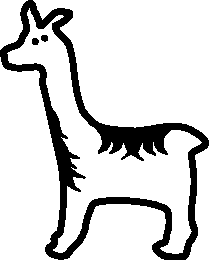
\includegraphics[height=1in]{../graphics/llama.pdf}
\]

Louie Llama is rather radical for a llama and doesn't mind being
rotated.

\begin{prob} 
Draw a picture of Louie Llama rotated $90^\circ$ counterclockwise.
\end{prob}

\begin{prob} 
Draw a picture of Louie Llama rotated $180^\circ$ counterclockwise.
\end{prob}

\begin{prob} 
Draw a picture of Louie Llama rotated $360^\circ$ counterclockwise.
\end{prob}

\begin{prob} Sometimes Louie Llama likes to walk around lines he finds:
\[
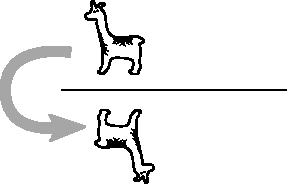
\includegraphics{../graphics/llamaLines.pdf}
\]
Through what angle did Louie Llama just rotate?
\end{prob}


Now we're going to watch Louie Llama go for a walk. Draw yourself any
triangle.  Actually, draw a crazy scalene triangle---those are the kind that Louie
Llama likes best. Louie Llama is going to proudly parade around this
triangle. When Louie Llama walks around corners he rotates. Check
it out:
\[
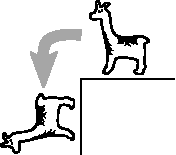
\includegraphics{../graphics/llamaCorner.pdf}
\]
Take your triangle and denote the measure of its angles as $a$, $b$,
and $c$. Start Louie Llama out along a side adjacent to the angle of
measure $a$. He should be on the outside of the triangle, his feet
should be pointing toward the triangle, and his face should be
pointing toward the angle of measure $b$.
\begin{prob} 
Sketch Louie Llama walking to the angle of measure $b$. Walk him
around the angle. As he goes around the angle his feet should always
be pointing toward the triangle. Through what angle did Louie Llama
just rotate?
\end{prob}

\begin{prob}
Sketch Louie Llama walking to the angle of measure $c$. Walk him
around the angle. Through what angle did Louie Llama just rotate?
\end{prob}

\begin{prob}
Finally, sketch Louie Llama walking back to the angle of measure
$a$. Walk him around the angle. He should be back at his starting
point. Through what angle did Louie Llama just rotate?
\end{prob}

\begin{prob} 
All in all, how many degrees did Louie Llama rotate in his walk?
\end{prob}

\begin{prob} 
Write an equation where the right-hand side is Louie Llama's total
rotation and the left-hand side is the sum of each rotation around the
angle. Can you solve for $a+b+c$?
\end{prob}

As you may have guessed, Louie Llama isn't your typical llama, for one
thing he likes to walk backwards and on his head! He also like to do
somersaults. Louie Llama can somersault around corners in two
different ways:
\[
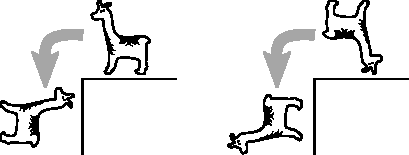
\includegraphics{../graphics/llamaSomer.pdf}
\]

\begin{prob} 
What does Louie Llama's somersault have to do with the angle of the
corner? Can you precisely explain how Louie Llama rotates when he
somersaults around corners?
\end{prob}


\begin{prob}
Can you walk Louie Llama around your original triangle, allowing him to
walk backwards (or even on his head!), letting him do somersaults as
he pleases around corners, and \textbf{directly} arrive at the
equation\index{triangle!sum of interior angles}
\[
a + b + c = 180^\circ?
\]
\end{prob}

\begin{prob} 
Can you rephrase what we did above in terms of \textit{exterior angles} and \textit{interior angles}?\index{interior angles}
\end{prob}

\break

\begin{prob} 
Can you walk Louie Llama around other shapes and figure out what the
sum of their interior angles are? Let's do this with a table:
\[
{\renewcommand{\arraystretch}{1.5}
\begin{tabular}{|c|c|c|}\hline
$n$-gon & sum of interior angles & interior angle of a regular $n$-gon\\\hline\hline
3 & & \\\hline
4 & & \\\hline
5 & & \\\hline
6 & & \\\hline
7 & & \\\hline
8 & & \\\hline
$n$ & & \\\hline
\end{tabular}}
\]
\end{prob}

